The fitness core in the processor architecture is the general processing core.
For genetic algorithms, the fitness core is tasked with calculating fitness scores for individuals, hence the name.

The design of the fitness core is highly influenced by the classic pipelined \gls{MIPS} core design ~\cite[p.~362]{compOrgDes}.
The core is designed as a five stage pipeline.
The contents of the different stages in the pipeline, however, differs from the original \gls{MIPS} architecture, as the CPU architecture has to accommodate for the \gls{ISA} design which combines ideas from multiple existing architectures.
An example of an \gls{ISA} feature which differs from \gls{MIPS} is the embedded branch-less conditionals\footnote{a feature which is shamelessly ripped whole-sale from ARM}.
An overview of the data path can be seen in figure \vref{fpga:fig:fitness:fitness_arch}.

\begin{figure}

  \centering
  % Trim er [left bottom right top]
  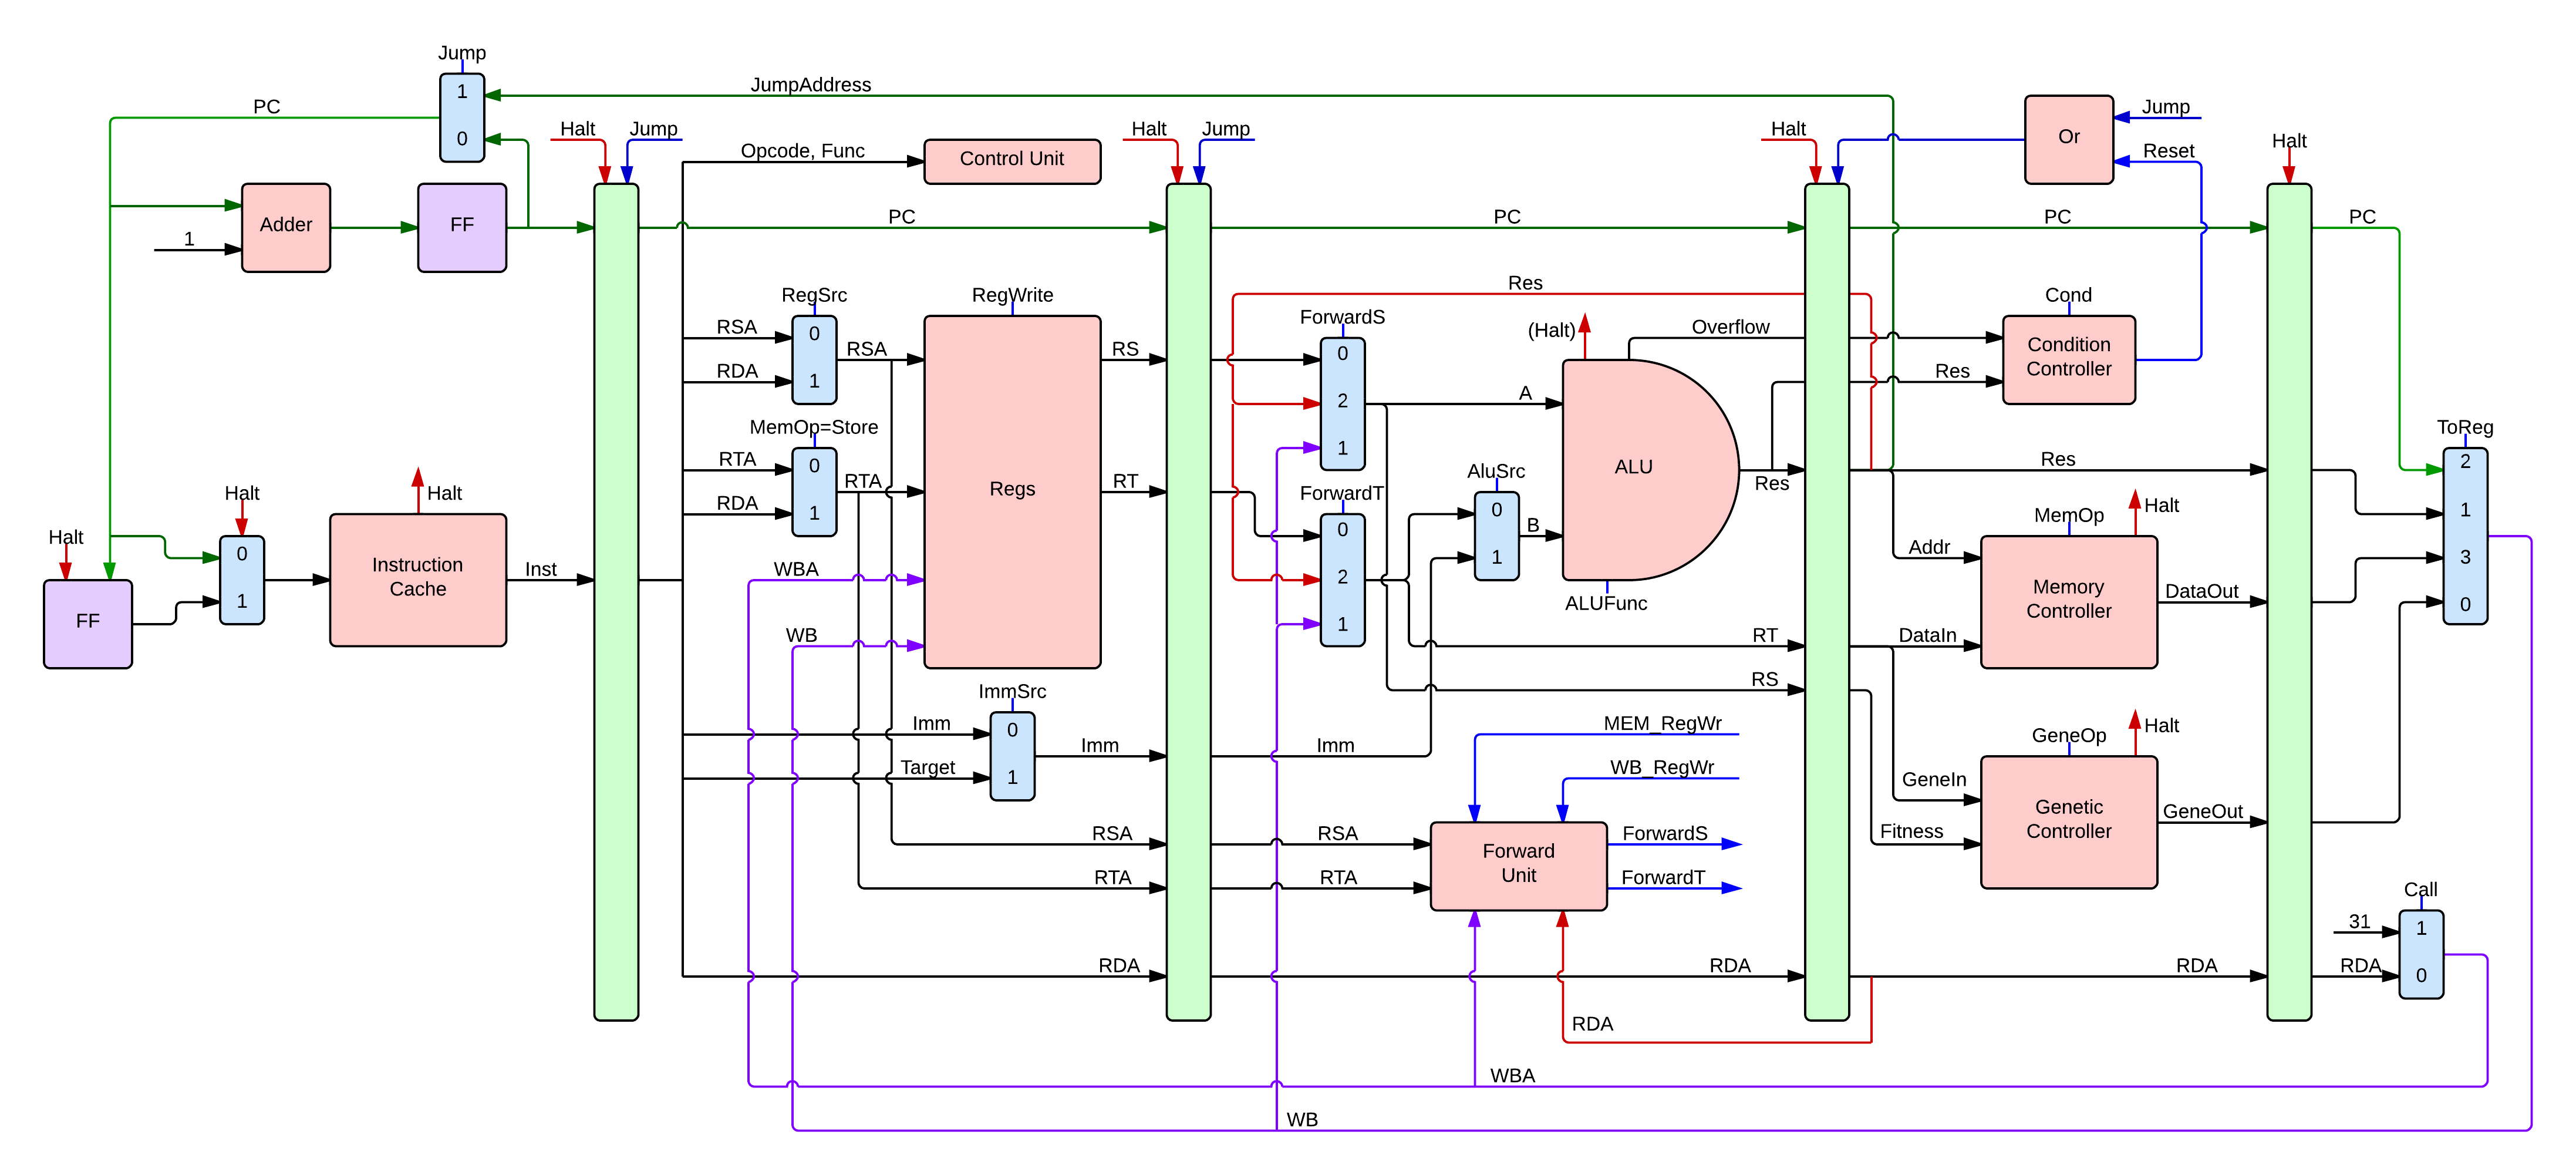
\includegraphics[width=\textwidth]{fpga/fig/fitness_core.png}
  \caption{Architecture block diagram}
  \label{fpga:fig:fitness:fitness_arch}
\end{figure}



The core is separated into several distinguable stages referred to as the \emph{fetch stage}, \emph{decode stage}, \emph{execution stage}, \emph{memory stage} and \emph{write-back stage}. These stages overlap in time and perform different tasks regarding the execution of instructions. The fetch stage is responsible for fetching a new instruction to the pipeline. The decode stage is responsible for decoding the instruction and set up the different control signals. The execution stage is involved in the actual computation of the instruction. The memory stage is responsible for performing memory related task on behalf of the instruction. The write-back stage is used to write data back into registers.

\todo{Review section}
 
\newpage
\subsubsection{Data Path} 

The data path is simple.
All instructions have the same length.
This makes it easier to fetch the instruction in the first stage and decode it in the second.
Also, the ISA only supports three different instructions classes with the register mappings located on the same positions.
This allows the register file to be read on the same time as the control unit determines the correct control signals for that particular instruction.
This allows for a shorter pipeline.
If the instruction format was asymmetric, the instruction would have to split the register file and decode stage in two stages.
A bigger pipeline would imply higher risk for pipeline hazards, and a more complicated hazard detection and correction schemes. 

The Barricelli computer is a load/store machine.
There is no preconception of a program stack at the hardware level.
This simplifies the execution and memory interaction.
Note that memory operands only appear in load and store instructions.
This implies that the execution stages is responsible for calculating the memory address and that the memory access can happen in the following stage.
Allowing the ALU to operate on operands in memory would expand the address stage, memory stage and the execution stage \cite[p.~335]{compOrgDes}.
The resulting architecture would involve a deeper pipeline. 


The MIPS inspired pipeline allows the design to be simple, but still powerful.
It  will increase performance by effectively increasing the instruction throughput.
Note that instruction throughput is an important metric because real applications execute millions of instructions \cite[p.~335]{compOrgDes}


The group decided that the overall design should be as simple as possible.
Hazard and branching schemes are kept simple.
Hazards are resolved with the \emph{forwarding unit}, which forwards data if dependencies are detected.
Branching are resolved with use of \emph{conditional} codes in each instructions.
The reader may refer to their respective sections for more details.

The fitness core features ``branch not taken'' branch prediction, which means that it assumes that conditional jumps will not be executed.
This gives a nice performance increase, because the pipeline does not have to be flushed when the branch is correctly predicted.
More advanced features like instruction rescheduling have not been implemented.

\newpage
\subsubsection{Control Unit} 

The control unit is the ``puppet master'' of the processor, so to speak.
Residing in the instruction decode stage, it is responsible for configuring all the different components for the current CPU operation so that the desired computation will emerge from the flow of data.
The control unit achieves this by setting the relevant control signals of the relevant components to the values associated with the current instruction.
Note that different instruction classes requires different use of the data path.
Thus, combinations the control signals must accommodate the different instructions formats. The different instructions classes and their corresponding control signals can be seen in table \ref{fpga:fitness:control_unit_out_tbl}. 

The control unit sets up the components based on the \emph{FUNCTION CODE} and the \emph{OPERATION CODE} of the instruction.
The \emph{FUNCTION CODE} is the 4 least significant bits of the instruction, and is responsible for determining the operation the ALU should perform. 

\begin{table}
    \centering
    \begin{tabular}{| l | c | c | c |c |}
    \hline
    Control signals   &              &          &                   \\[0.5ex]
                      & RRR          & JUMP     &  SW   &  STG       \\
    \hline
    ALU\_SOURCE       &              &          &       &            \\
    IMM\_SOURCE       &              &          &       &            \\
    REG\_STORE        &              &          &       &            \\
    STORE\_SOURCE     &              &          &       &            \\
    CALL              &              &          &       &            \\
    JUMP              &              &          &       &            \\
    GENE\_OP          &              &          &       &            \\
    MEM\_OP           &              &          &       &            \\
    TO\_REG           &              &          &       &            \\
    \hline  
                      & RRI          & LW       & STI   & SETG       \\
    \hline
    ALU\_SOURCE       &              &          &       &            \\
    IMM\_SOURCE       &              &          &       &            \\
    REG\_STORE        &              &          &       &            \\
    STORE\_SOURCE     &              &          &       &            \\
    CALL              &              &          &       &            \\
    JUMP              &              &          &       &            \\
    GENE\_OP          &              &          &       &            \\
    MEM\_OP           &              &          &       &            \\
    TO\_REG           &              &          &       &            \\
    \hline
                      & CALL         & LDI      & LDG   &            \\
    \hline  
    ALU\_SOURCE       &              &          &       &            \\
    IMM\_SOURCE       &              &          &       &            \\
    REG\_STORE        &              &          &       &            \\
    STORE\_SOURCE     &              &          &       &            \\
    CALL              &              &          &       &            \\
    JUMP              &              &          &       &            \\
    GENE\_OP          &              &          &       &            \\
    MEM\_OP           &              &          &       &            \\
    TO\_REG           &              &          &       &            \\   
    \hline
    \end{tabular}
    \caption{Control unit output}
    \label{fpga:fitness:control_unit_out_tbl}

\end{table}

 
\begin{table}[h]
    \centering
    \begin{tabular}{| l | l |}
    \hline
    Opcode & Instruction class \\
    \hline
    1000   & RRR               \\
    1100   & RRI               \\
    0000   & LW                \\
    0001   & SW                \\
    0100   & LDI               \\
    0010   & JMP               \\
    0011   & CALL              \\
    0101   & STI               \\
    1001   & LDG               \\
    1010   & SETG              \\
    1011   & STG               \\
    \hline       
    
    \end{tabular}
    \caption{Overview of opcodes}
    \label{fpga:tbl:opcode_tbl}

\end{table}


\input{fpga/tbl/fitness_core_control_unit_tbl}

%%The meaning of the different control signals

The following paragraphs exhaustively documents and explains the technical details of each of the control unit's control signals.

\paragraph{ALU\_FUNC}
The \emph{ALU\_FUNC} is the least four significant bits of the instruction, and is responsible for determining the type of operation the \emph{ALU} should perform.
This are set according to table \ref{fpga:tbl:alu_function_codes_tbl} 

\begin{savenotes}
\begin{table}
\centering
    \begin{tabular}{| l | l |}
     \hline
     FUNC code & operation \\
     0000      & ADD       \\
     0001      & SUB       \\
     0010      & MUL       \\
     0011      & SRA       \\
     0100      & OR        \\
     0101      & AND       \\
     0110      & XOR       \\
     0111      & SLL       \\
     1000      & SRL       \\
     1001      & OP1 \footnote{Gives input 1 as output.}       \\
     1010      & OP2 \footnote{Gives input 2 as output.}      \\
     1111      & NOP       \\
     \hline
   \end{tabular}
    \caption{Overview of function codes}
    \label{fpga:tbl:alu_function_codes_tbl}



\end{table}
\end{savenotes}

\paragraph{ALU\_SOURCE}
The \emph{ALU\_SOURCE} signal is used to specify the second \emph{ALU operand}.
When this signal is asserted the second ALU operand is the immediate field of the instruction.
This implies that the instruction class of the instruction is either RRI or RI.
On the other hand, if this signal is de-asserted, the operand comes from read register to of the instruction file. Note that this value may or may not have been forwarded. 

\paragraph{REG\_WRITE}
This signal specifies whether the write back value residing in the \emph{write-back} stage should be written to the register file.
When this signal is asserted, the value from the \emph{write-back} stage is written to the specified register address.
The register address is specified in the instruction, and always resides in the RT address field of the instruction.

\paragraph{IMM\_SOURCE}
The \Gls{galapagos} ISA has two different instruction classes (RI, RRI) that uses different lengths of the immediate field.
In order to differentiate between these immediate fields, the \emph{IMM\_SOURCE} signal is responsible for selecting the correct immediate field based on the instruction class of the current instruction.
The selection is done with a multiplexer.
In the case of an RRI instruction the 10-bits immediate field is selected, and in the case of an RI instruction, the 19-bits field is chosen.

\paragraph{REG\_SOURCE}
For \emph{JMP} and \emph{CALL} instructions, the immediate address field of the instruction is added with the address content of Rd.
The Rd address specified in the instruction must be read from the register file.
Normally, the register file would use the \emph{Rs} and \emph{Rt} part of the instructions as inputs to the register file.
In the special case of \emph{RI} instructions the register file must read the Rd instead of Rs.
This is accomplished by asserting the \emph{REG\_SOURCE} signal, which causes a multiplexer to choose the \emph{Rd} portion of the instruction instead of the \emph{Rs} as input to the register file.
This will output the content of the correct data from the register file.
This is visible in figure \todo{reference figure}.


\paragraph{STORE\_SOURCE}
For the \emph{ST} instruction, the register address of the data to be stored is located in the \emph{Rd} field of the instruction.  Normally, the register file would use the \emph{Rs} and \emph{Rt} part of the instruction as inputs to the register file. In the special case of a \emph{ST} instruction the register file must read the \emph{Rd} register instead of \emph{Rt}. This is accomplished by asserting the \emph{MEM\_WRITE} signal, which causes a multiplexor to chose the \emph{Rd} portion of the instruction instead of the \emph{Rt} as input to the register file. 

This will output the content of the correct data from the register file. This ensures that the \emph{Rt} signal seen in \ref{fpga:fig:fitness:fitness_arch} contains the content of the \emph{Rd} register. This is actually the data that is written to memory.

\todo{Review this section}



\todo{this}

\paragraph{JUMP}
The JMP instruction uses the address in the immediate field of the instruction to load a new value into the \emph{program counter} register.
The jump signal selects between the jump address and the incremented program counter when deciding a new value for the program counter at each cycle.
In case of jump, this signal is asserted and the jump address is chosen.
When de-asserted the program counter is set to the incremented program counter, making the program execute normally.
This signal is also asserted when performing call instructions.   

\paragraph{CALL}
The \Gls{galapagos} ISA supports non-recursive procedure calls at a hardware level.
The call instruction works similar to the jump instruction described above.
The difference is that the incremented value of the program counter before the jump is stored to register r31, which is conventionally used as a link register.
This value can be used later when returning from the procedure call.
To return from a procedure call, one  needs simply to jump back to the address stored in r31.

The \emph{CALL} signal is responsible for making sure that the incremented program counter is stored at register 31.
When asserted the signal make sure that the write register address is changed to 31.
If the signal is de-asserted the write register will stay unmodified, and the Rt register in the instruction is responsible for specifying the register address.


\paragraph{GENE\_OP}
Loading and storing of fitness values and chromosomes is the responsibility of the \emph{genetic controller}.
This controller is able to perform three types of actions: \emph{load}, \emph{store} and \emph{settings}, dependent of the instruction class executed.
When performing a load, a chromosome is loaded from the unrated pool.
The store operation is used to store a chromosome and its corresponding fitness value to the rated pool.
The settings are used to apply settings to the genetic pipeline.
In order to divide these cases, the Galapagos architecture relies on the \emph{gene operation} vector.
This bit-vector is set depending on the instruction class as seen in table \ref{fpga:tbl:gene_op_code_tbl}.

\begin{table}[h]
\centering
    \begin{tabular}{| l | l | l |}
     \hline
     Code  & Meaning      & Instruction class \\
     \hline
     00    & NOP          &   OTHER           \\
     01    & LOAD\_GENE   &   LDG             \\
     10    & STORE        &   STG             \\
     11    & SETTINGS     &   SETG            \\
    \hline
    \end{tabular}
    
    \caption{Gene operation codes}
    \label{fpga:tbl:gene_op_code_tbl}
    

\end{table}


Depending on the bit-vector-signal, the \emph{genetic controller} is able to perform the appropriate action. 

\paragraph{MEM\_OP}
As with the genetic controller, the memory controller must be able to distinguish between operations.
In case of memory controller, these operations are loading and storing to and from the external data memory.
These signals are set according to the instruction class currently being executed.
An overview can be found in table \ref{fpga:tbl:mem_op_code_tbl}

\begin{table}[h]
\centering
    \begin{tabular}{| l | l | l |}
     \hline
     Code  & Meaning      & Instruction class \\
     \hline
     00    & NOP          &   OTHER          \\
     01    & LOAD\_DATA   &   LW             \\
     10    & STORE\_DATA  &   SW             \\
    \hline
    \end{tabular}
    
    \caption{Memory operation codes}
    \label{fpga:tbl:mem_op_code_tbl}
    

\end{table}


\paragraph{TO\_REG}
In the \emph{write-back} stage, there is need to distinguish between several outputs from the \emph{memory stage}.
The \emph{TO\_REG} signal is responsible for selecting which value that should be written to the register file.
The selection is aided by a 4-to-1 multiplexer.
The different inputs are: \emph{Gene}, \emph{Data}, and \emph{PC+1}, \emph{Res}, as seen in figure \todo{add reference}.
However, keep in mind that the \emph{REG\_WRITE} signals must be asserted for the data to be written. 

The \emph{TO\_REG} bit-vector are set according to table \ref{fpga:tbl:to_reg_multiplexor_output_tbl}

\begin{savenotes}
\begin{table}[h]
\centering
    \begin{tabular}{| l | l | l |}
     \hline
     Code  & Output       & Instruction class \\
     \hline
     00    & GENE      &   LDG                \\
     01    & RES       &   OTHER \footnote{OTHERS refers to instructions that store the ALU result to a register }             \\
     10    & PC+1      &   CALL              \\
     11    & DATA      &   LW                \\
    \hline
    \end{tabular}
    
    \caption{4-to-1 multiplexor output}
    \label{fpga:tbl:to_reg_multiplexor_output_tbl}
    

\end{table}
\end{savenotes}


\newpage
\subsubsection{The ALU}

The Arithmetic Logic Unit, or ALU, is the heart of the fitness core, colloquially put.
It is responsible for executing scheduled arithmetic and logical operations on data.
The ALU is perhaps the single most important component of the fitness core.

The ALU in the fitness core is capable of performing a large array of different mathematical and logical operations on 64-bit words, including addition, subtraction, comparisons, shifts and multiplications, in addition to a slew of bitwise logical operations such as and, or, xor and not.
Division is not supported.

On the FPGA, large parts of the ALU is implemented with \glspl{DSP slice}, which means that dedicated pre-fabricated ALU-specific circuitry is used in place of regular generic \gls{FPGA} \glspl{LUT} for increased performance and space utilization.

\paragraph{Multiplication}

Multiplication is handled as a special case in the architecture.
The multiplication is designed to use two cycles in the \emph{execution stage}, rather than the normal one cycle per operation.
This is because the multiplication is the slowest of the ALU operations, and the maximum clock frequency would be severely limited, were the multiplication path allowed to become the longest path.
This would result in a degradation of the overall performance of the processor, which is not desirable.
To overcome this limitation, a state machine is designed in the execution stage to halt the pipeline when performing multiplication.
This effectively makes the multiplication a multi-cycle operation.
The result of this is that the multiplication operation is able to finish without the rest of the system needing to slow down to accommodate for it, meaning that the maximum clock speed is not limited by the multiplication circuitry.

\paragraph{Shifters}

A shifter is a subcomponent within the ALU designed for efficient generic bit shifting.
A shifter can shift an input by \emph{M} bits, either left or right unsigned, or right signed. \emph{M} is set generically when the component is created, while signal inputs  \emph{Left} and \emph{Arith} determines type of shift. 
If \emph{Left} is set, there is unsigned shift to left.
If \emph{Left} is not set, but \emph{Arith} is, then it is a signed shift to right.
Otherwise, the shift is to the right unsigned.
If \emph{Enable} is not set, then there will be no shift.

\paragraph{ShifterVariables}
A ShifterVariable consists of a larger set of shifters. 
It takes two inputs: One main input \emph{I} with size \emph{N} (default 64) to be shifted, and a \emph{count} input of size \emph{M} that determines how many bits to be shifted. 
\emph{M} should be $log_2$ of \emph{N}. 
The number of shifters in the ShifterVariable is equal to \emph{M} (default 1), and each shifter \emph{i} may shift the main input by $2^i$ bits, where \emph{i} is a number in the range 0 to M-1. 
Total shift is $\sum_{i=0}^{M-1} count_i * 2^i$ where $count_i$ is bit number \emph{i} in the \emph{count} input.
For example, if it is 000110, shift of input \emph{I} is $0*2^5 + 0*2^4 + 0*2^3 + 1*2^2 + 1*2^1 + 0*2^0 = 2^2 + 2^1 = 6$.
This can be seen in figure \vref{fig_shifter}
\begin{figure}[H]
\center
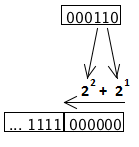
\includegraphics[width=0.3\textwidth]{fpga/fig/shift.png}
\caption{Example use of ShifterVariable}
\label{fig_shifter}
\end{figure}

The ShifterVariable has also inputs for \emph{Left}, \emph{Arith} and \emph{Enable} for each shifter.
ShifterVariables are not only used in the ALU, but also in the Crossover Core and Mutation Cores in the Genetics Pipeline.

\newpage
\subsubsection{Forwarding Unit} \label{fpga:fitness:sss:forwarding_unit}
Since the execution of instructions overlap in the pipeline, there is need for some mechanism to handle the data dependencies that arise between the instructions.
These dependencies are known as data hazards.
They occur when a planned execution of an instruction cannot happen in that cycle because some data is not yet available.
This problem can be solved in two ways, either by stalling or forwarding.
Stalling, the simplest solution, is done by avoiding the hazard by stalling until the data becomes available.
This is accomplished by inserting \emph{NOPs} in the pipeline.
Although, this method works, it is unacceptably slow for a high performance architecture.
Since this processor aims to achieve high performance, stalling is far from optimal.
A far better approach is to rely on register forwarding.
In this approach the aim is to resolve the dependencies by simply forwarding internal resources from one pipeline stage to another, if needed.

The forwarding logic is implemented by comparing register dependencies of the currently executing instruction with the other instructions currently flowing through the pipeline.
If the forwarding unit detects a data hazard, it will forward the appropriate data to the execution stage so it can be used at once.
An overview of the control signals and their meaning can be seen in table. \ref{tbl:fpga:forwarding_signals}.

A second, more unconventional forwarding unit is also implemented in the decode stage.
It forwards data from the write back stage to the decode stage to solve data hazards caused by a single cycle write delay in the register file that the regular forwarding unit cannot detect.

Unfortunately, forwarding does not solve all possible data hazards in the processor.
In the case of a memory load instruction being immediately proceeded by an instruction dependant on the data fetched from memory, a data hazard occurs.
Since it does not make sense to forward data from memory, this class of data hazards is resulted by stalling.
The Galapagos architecture does not solve this problem in hardware, but rather in software.
The assembler is responsible for inserting \emph{NOP} instructions in case of such hazards.  

\begin{table}[H]
    \centering
    \begin{tabular}{| p{2.5cm} p{9cm} |}
    \hline
    Control signal  & Meaning \\ [0.5ex]
    \hline 
    forwardA=00  & The first ALU operand is from the register file\\
    
    forwardA=10  & The first ALU operand is from the prior ALU result\\
    
    forwardA=01  & The first ALU operand is either data from memory or an earlier ALU      result\\
    
    & \\
    forwardB=00  & The second ALU operand is from the register file\\
    forwardB=10  & The second ALU operand is from the prior ALU result \\
    forwardB=01 & The second ALU operand is either data from memory or an earlier ALU result \\
    \hline
    \end{tabular}
    \caption{Forwarding control signals}
    \label{tbl:fpga:forwarding_signals}

\end{table}


\newpage
\subsubsection{Conditional Unit}
Like ARM, the \Gls{galapagos} architecture embeds conditional codes in every single instruction in order to determine if it should be executed.
In Barricelli's processor, every instruction is executed, but the conditional codes may disable the effect of the instruction.
The \emph{condition unit} is responsible for checking the condition code against the status flags set by the previous instruction, and using this information to effect the conditional.

\newpage
\subsubsection{Fitness Memory Controller} 
In order to communicate with the main data controller, each fitness cores contains a small version of the data controller to synchronize the communication to the main controller.
This small controller, referred to as the \emph{fitness data memory controller}, is responsible for mediating memory requests between the data memory controller and the fitness memory controller.

To use the data memory bus, the the \emph{fitness memory controller} may send a request signal to the main \emph{Data controller}. 
The \emph{data controller} either handles this request immediately, or the request is handled when the bus is ready, in case some other core is currently using the bus.
Either way, the requesting fitness core will halt the pipeline waiting for access to the bus.
When the \emph{data controller} is ready, it will send out an acknowledgment granting the bus.
Upon receiving the bus, the \emph{fitness memory controller} is able to use it freely. 

In case of a \emph{READ} operation, the address is put on the address bus. This address corresponds to a memory position on the external memory. When receiving this address, the \emph{data memory controller}, starts fetching the memory word. During this time the fitness memory controller needs to wait. It stays in a wait loop unit the \emph{data memory controller} is finished reading. Note that the bus to external memory is only 16-bits wide. This implies that four read instructions are required to read a 64-bits word. When the \emph{memory data controller} is finished reading data from memory, the data is put on the data bus, and the can be read by the fitness core. Then the fitness core is disconnected from both the data and memory bus and it continuous its execution through the pipeline.


When performing a \emph{WRITE} operation this is done in the same manner as with the \emph{READ} operation. The difference lay in the fact that during a memory write, the data to be written is put on the outgoing data bus. The \emph{fitness core} is in wait state at this moment. When the data is finished writing to memory, the \emph{memory data controller} responds with an acknowledgement. The \emph{fitness core} continuous with its computation.  
A state diagram showing this can be seen in figure \ref{fpga:fitness:fitness_memory_ctrl}.  

\todo{Review this section} 


\begin{figure}[H]
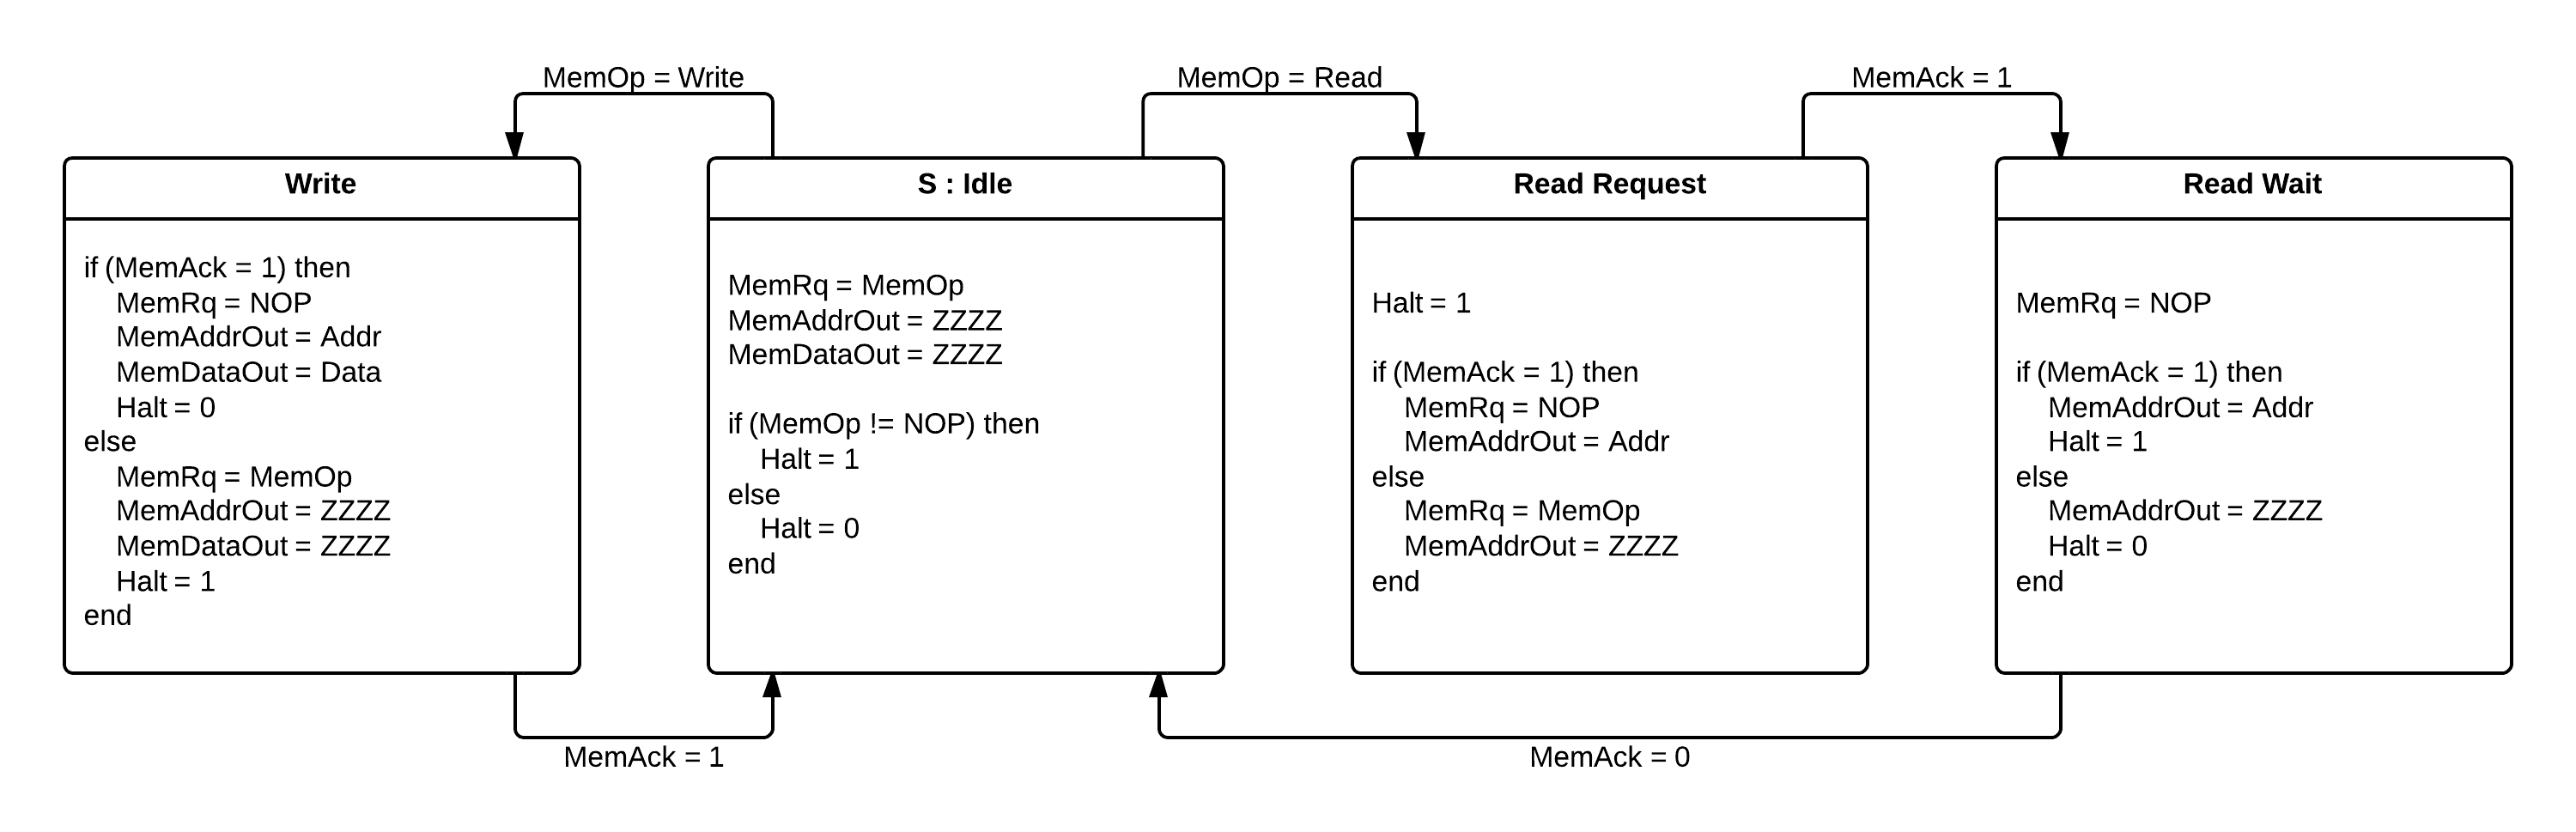
\includegraphics[width=\textwidth]{fpga/fig/fitness_mem_ctrl.png}
\caption{Fitness memory controller state machine}
\label{fpga:fitness:fitness_memory_ctrl}
\end{figure}



\newpage
\subsubsection{Fitness Genetic Controller} 

Analogously to the fitness core, the genetics pipeline also has a separate mediating memory controller.
This controller is referred to as the \emph{fitness genetic controller}.
It is more complex than its sibling in the fitness core, since it interfaces with the genetics data controller, which arbitrates two independent memory stores. This controller is very similar the \emph{fitness data controller}. The difference lays in the fact that two values are transferred in case of \emph{WRITE} operations. The protocol itself is mostly similar. The a state diagram showing the inner workings of this controller can be seen in figure \ref{fpga:fitness:fitness_genetic_ctrl}. 

\todo{review this section}


\begin{figure}[H]
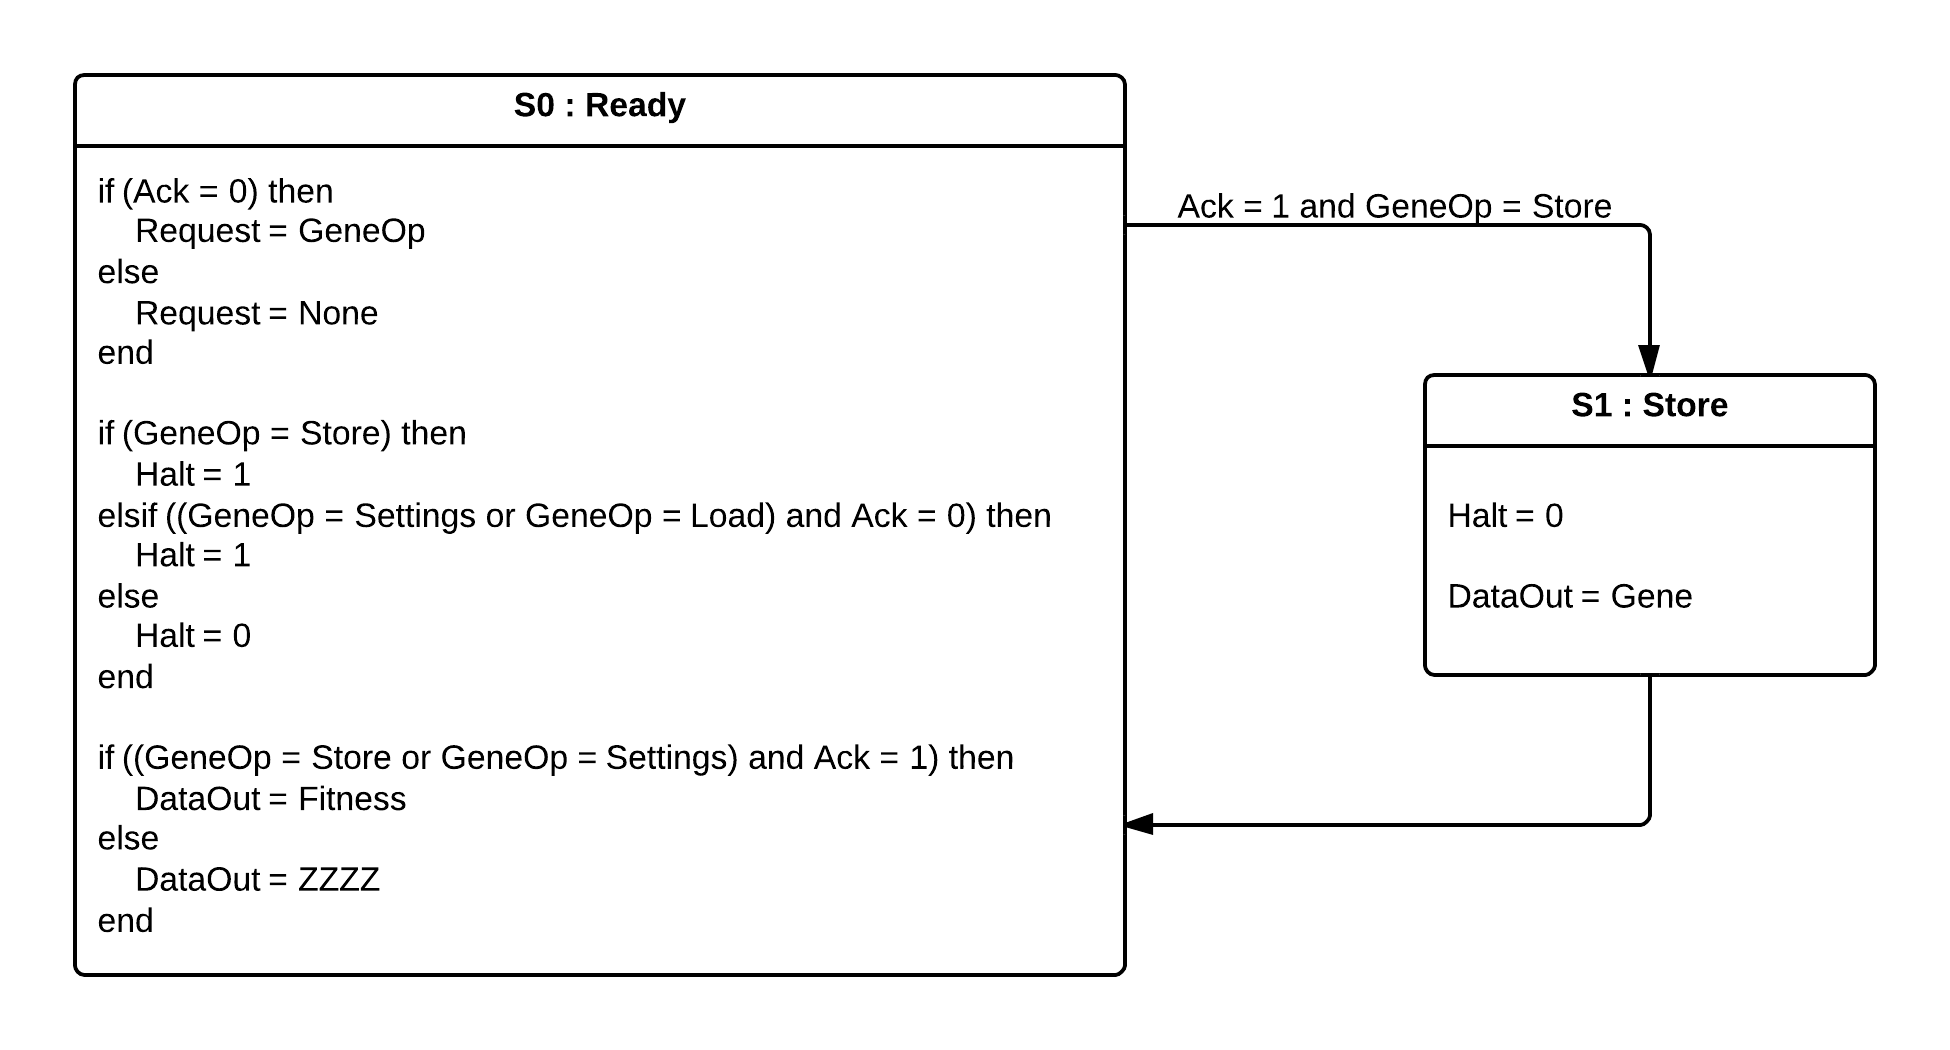
\includegraphics[width=\textwidth]{fpga/fig/fitness_genetic_ctrl.png}
\caption{Fitness genetic controller state machine}
\label{fpga:fitness:fitness_genetic_ctrl}
\end{figure}


\newpage
\subsubsection{Halting the Pipeline}

In normal computer systems, the time to access the memory is variable.
It depends on the different states of the machine.
This imposes a problem when several cores competes about access to the memory.
It is difficult to determine precisely the times that is actually used to receive the required data.
In order to fix this issue, and to prevent the processor to compute when there is no data, each interaction with memory is able to halt the processor if need be.
The different situations arise when accessing the instruction memory, data memory, and the genetic data pools.
Their corresponding controllers are able to set a halt signal before performing the operation.
When the one of the \emph{halt} signals is asserted, the program counter and the pipeline registers will be halted, ensuring that the \emph{fitness core} does not change state prematurely. 
